%\documentclass[]{beamer}
\documentclass[handout]{beamer}
%\usepackage[dvips]{color}
\usepackage{graphicx}
\usepackage{amsmath,amssymb,array,comment,eucal}
\input{../macros}
\usepackage{verbatim}

\usetheme{Warsaw}
\usecolortheme{orchid}
\title{Choice of Prior Distributions}
\institute{Merlise Clyde}
\author{STA721 Linear Models Duke University}
\date{September 17, 2015}
\logo{duke.eps}

\begin{document}
\maketitle

\begin{frame}
  \frametitle{Bayesian Estimation}
  Model 
$$
\Y \sim \N(\X \b, \I_n/\phi)
$$
precision  $\phi = 1/\sigma^2$ 
\pause

\vspace{14pt}
Normal-Gamma Conjugate prior  $\NG(\bv_0, \Phi_0, \v_0, \SS_0)$
  \begin{eqnarray*}
\Phi_n & = & \X^T\X +  \Phi_0  \\
\bv_n &  = & \Phi_n^{-1} (\X^T\X \bhat  + \Phi_0 \bv_0)  \\
\nu_n  & = & \nu_0 + n   \\
\SS_n & = & \SSE + \SS_0 + \bhat^T \X^T\X \bhat + \bv_0^T \Phi_0 \bv_0
 - \bv_n^T \Phi_n \bv_n   \\
\hat{\sigma}^2_n & \equiv & \SS_n/\nu_n \pause
  \end{eqnarray*}

Posterior Distribution
  \begin{eqnarray*}
\b \mid \phi, \Y & \sim &\N(\bv_n, (\phi \Phi_n)^{-1}) \pause \\
\phi \mid \Y &\sim &\G(\frac{\nu_n}{2}, \frac{  \nu_n \hat{\sigma}^2_n}{2})
  \end{eqnarray*}
  

\end{frame}


\begin{frame}
  \frametitle{Marginal Distribution from Normal--Gamma }
  \begin{theorem}
    Let  $\t \mid \phi \sim \N(m, \frac{1}{\phi} \Sigma)$ and $\phi \sim
    \G(\nu/2, \nu \shat/2)$. Then  $\t$ ($p \times 1)$ has a $p$
    dimensional multivariate $t$ distribution $$\t \sim t_\nu( m,
    \shat \Sigma )$$ with density
$$p(\t) \propto  \left[ 1 + \frac{1}{\nu}  \frac{ (\t - m)^T
    \Sigma^{-1} (\t - m)}{\shat} \right]^{- \frac{p + \nu}{2}}$$
  \end{theorem}
\end{frame}


\begin{frame}
  \frametitle{Marginal Posterior Distribution of $\b$}
  \begin{eqnarray*}
\b \mid \phi, \Y  & \sim & \N( \bv_n, \phi^{-1} \Phi_n^{-1}) \pause \\    
 \phi \mid \Y & \sim & \G\left(\frac{\nu_n}{2},  \frac{\SS_n}{ 2} \right) 
  \end{eqnarray*}
\pause

Let $\shat = \SS_n/\nu_n$  (Bayesian MSE) \pause

Then the marginal posterior distribution of $\b$ is 
$$
\b  \mid \Y \sim t_{\nu_n} (\bv_n, \shat \Phi_n^{-1})
$$ \pause


Any linear combination $\lambda^T\b$
$$\lambda^T\b  \mid \Y \sim t_{\nu_n}
(\lambda^T\bv_n, \shat \lambda^T\Phi_n^{-1}\lambda)$$ has a univariate
$t$ distribution with $\v_n$ degrees of freedom

\end{frame}

\begin{frame}
  \frametitle{Predictive Distribution}
Suppose $\Y^* \mid \b, \phi \sim \N(\X^* \b , \I/\phi)$  and is conditionally
independent of $\Y$ given $\b$ and $\phi$ \pause
\vspace{18pt}

What is the predictive distribution of $\Y^* \mid \Y$? \pause

\vspace{18pt}
$\Y^* = \X^* \b + \eps^*$ and $\eps^*$ is independent of $\Y$ given
$\phi$ \pause

\begin{eqnarray*}
\X^* \b + \eps^* \mid \phi, \Y & \sim & \N(\X^*\bv_n, (\X^{*} \Phi_n^{-1} \X^{*T}
+ \I)/\phi)  \pause \\
\Y^* \mid \phi, \Y & \sim & \N(\X^*\bv_n, (\X^{*} \Phi_n^{-1} \X^{*T}
+ \I)/\phi)  \pause \\
\phi \mid \Y & \sim & \G\left(\frac{\nu_n}{2},
  \frac{\shat \nu_n}{ 2} \right)  \pause \\
\Y^* \mid \Y & \sim & t_{\nu_n}( \X^*\bv_n, \shat (\I + \X^* \Phi_n^{-1} \X^T))
\end{eqnarray*}
\end{frame}
\begin{frame}
  \frametitle{Alternative Derivation}
Conditional Distribution:
\begin{eqnarray*}
f(\Y^* \mid \Y) & = & \frac{f(\Y^*, \Y)}{f(\Y)} \pause \\
 & = & \frac{
\iint f(\Y^*, \Y \mid \b, \phi) p(\b, \phi) d\b\, d\phi
}
{
  f(\Y)
}  \pause \\
 & = & \frac{
\iint f(\Y^*\mid \b, \phi) f(\Y \mid \b, \phi) p(\b, \phi) d\b\, d\phi
}
{
  f(\Y)
}  \pause \\
 & = & 
\iint f(\Y^*\mid \b, \phi)  p(\b, \phi \mid \Y) d\b\, d\phi \pause
\end{eqnarray*}
Complete the''Square'' or quadratic to integrate out $\b$, then integrate out $\phi$
\end{frame}

\begin{frame}
  \frametitle{Conjugate Priors}
  \begin{definition}
    A class of prior distributions $\cP$ for $\t$ is conjugate for a
    sampling model $p(y \mid \t)$ if for every $p(\t) \in \cP$, $p(\t
    \mid \Y) \in \cP$.
  \end{definition}
\pause  
  Advantages: \pause
  \begin{itemize}
  \item Closed form distributions for most quantities; bypass MCMC for
    calculations \pause
  \item Simple updating in terms of sufficient statistics ``weighted
    average'' \pause
  \item Interpretation as prior samples - prior sample size \pause
  \item Elicitation of prior through imaginary or historical data \pause
  \item limiting ``non-proper'' form recovers MLEs \pause
  \end{itemize}
Choice of conjugate prior?
\end{frame}

\begin{frame}
  \frametitle{Unit Information Prior}

Unit information prior $\b \mid \phi \sim \N(\bhat, n
   (\X^T\X)^{-1}/\phi)$ \pause
  \begin{itemize}
\item Fisher Information is $\phi \X^T\X$ based on a sample of $n$
  observations \pause
\item Inverse Fisher information is covariance matrix of MLE \pause
\item ``average information'' in one observation is  $\phi \X^T\X /n$ \pause
\item center prior at MLE and base covariance on the information in
  ``1'' observation \pause
\item  Posterior mean 
$$\frac{n}{1 + n} \bhat +  \frac{1}{1 + n}\bhat = \bhat$$ \pause
\item Posterior Distribution 
$$\b \mid \Y, \phi \sim \N\left( \bhat, \frac{n}{1 + n} (\X^T\X)^{-1}
  \phi^{-1} \right)$$ \pause
    \end{itemize}
Cannot represent real prior beliefs; double use of data but has the
``right'' behaviour.  
\end{frame}

\begin{frame}
  \frametitle{Zellner's $g$-prior}
Zellner's g-prior(s) $\b \mid \phi \sim \N(\bv_0, g
    (\X^T\X)^{-1}/\phi)$ \pause

$$\b \mid \Y, \phi \sim \N\left( \frac{g}{1 + g} \bhat +  \frac{1}{1 + g}
\bv_0, \frac{g}{1 + g} (\X^T\X)^{-1} \phi^{-1} \right)$$ \pause

\begin{itemize}
\item Invariance: Require posterior of   $\X \b$  equal the posterior of $\X \H \alphav$
\pause   ($\a_0 = \H^{-1} \bv_0$)  ( take $\bv_0 = \zero$)

\item Choice of $g$?  \pause
\item $\frac{g}{1 + g}$  weight given to the data \pause
\item Fixed $g$ effect does not vanish as $n \to \infty$ 
\item Use $g = n$ or place a prior distribution on $g$
\end{itemize}


\end{frame}
\begin{frame}
  \frametitle{Shrinkage}
 Posterior mean under  $g$-prior  with $\bv_0 = 0$
$\frac{g}{1 +g} \bhat $

\centerline{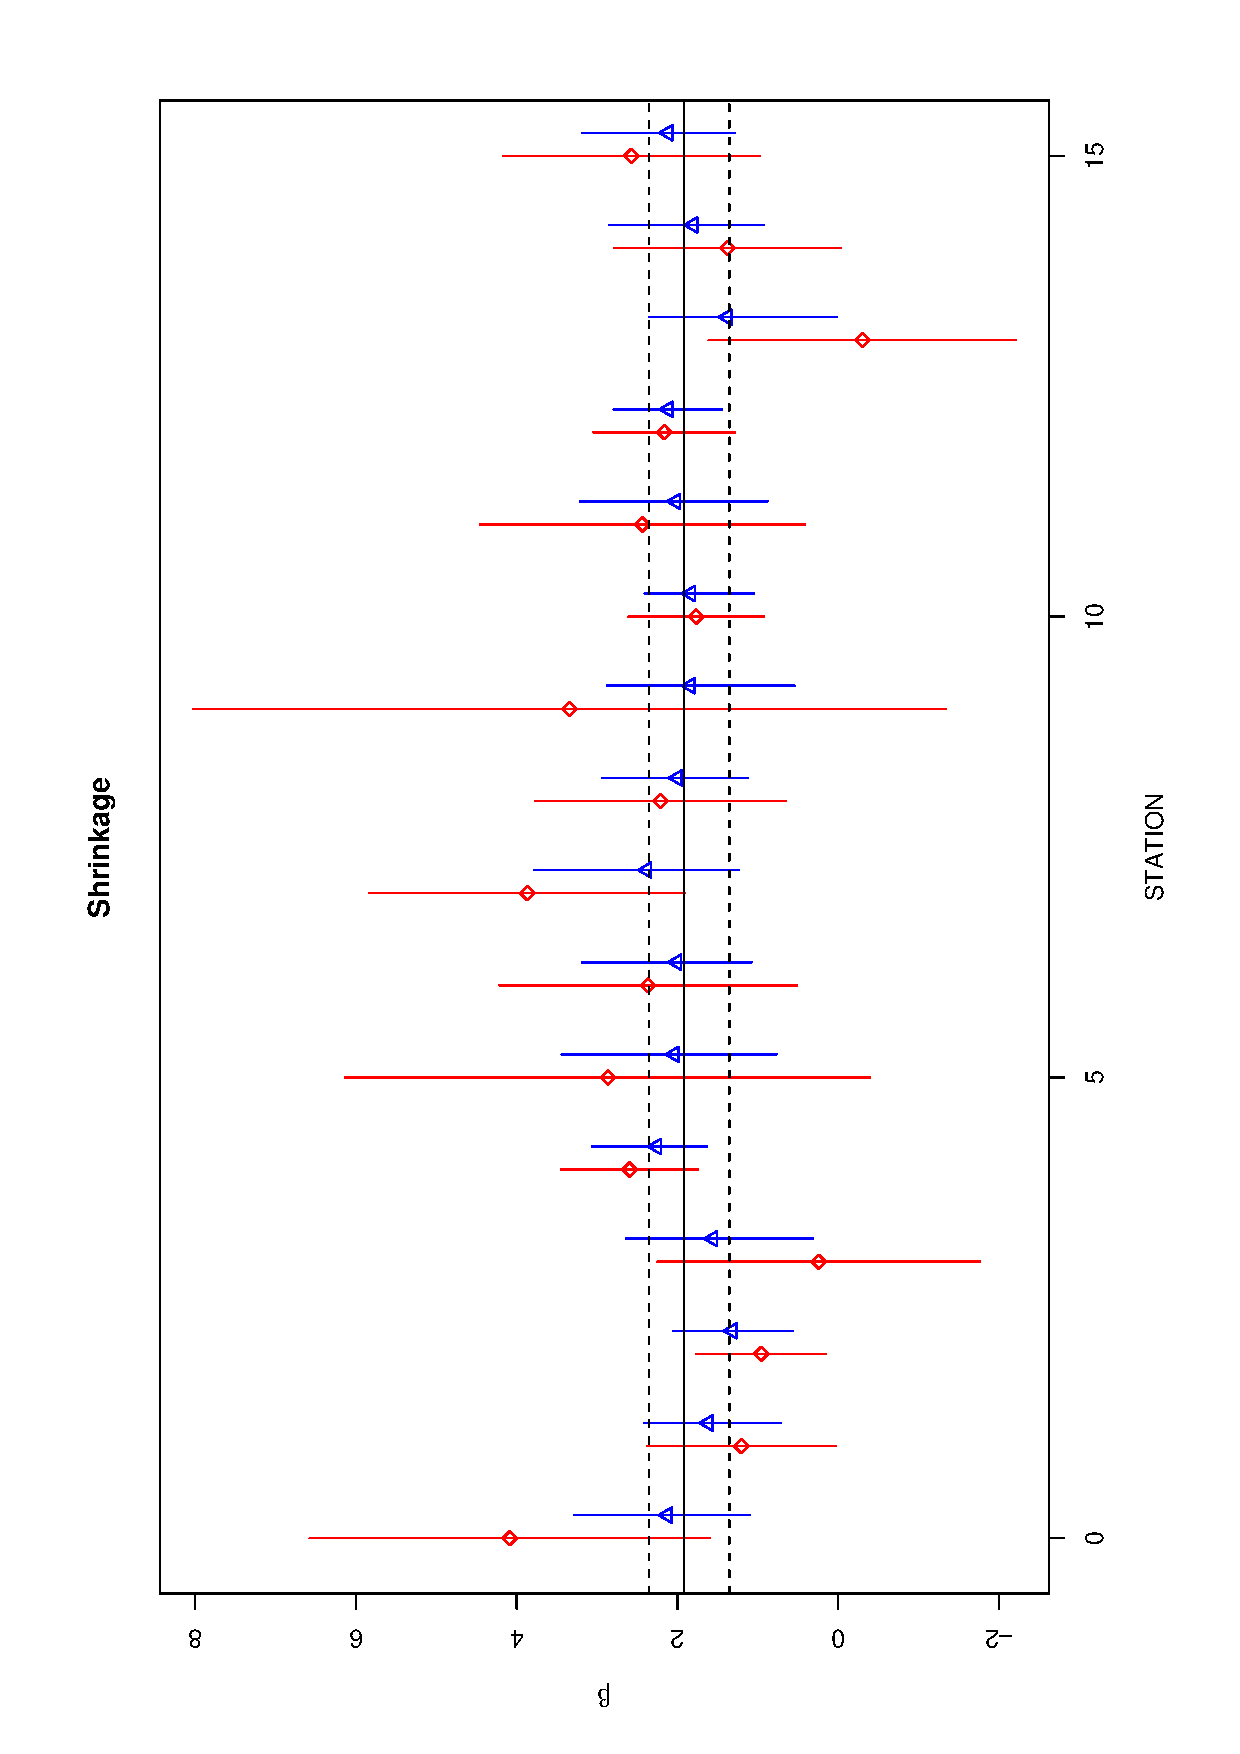
\includegraphics[height=3in]{shrinkage}}
\end{frame}


\begin{frame}
  \frametitle{Jeffreys Prior}
  
Jeffreys proposed a default  procedure so that resulting prior
would be invariant to model parameterization  \pause

$$p(\t) \propto |\cI(\t)|^{1/2}$$
\pause
where $\cI(\t)$ is the  Expected Fisher Information matrix
\pause
$$
\cI(\theta) = - \E[ \left[ \frac{\partial^2 \log(\cL(\t))}{\partial
  \theta_i \partial \theta_j} \right] ]
$$
\end{frame}
\begin{frame}
  \frametitle{Fisher Information Matrix}
Log Likelihood
$$
    \log(\cL(\b, \phi))  =  \, \frac{n}{2} \log(\phi)  - \frac{\phi}{2}
     \| (\I - \P_\x) \Y\|^2  
 - \frac{\phi}{2}(\b - \bhat)^T(\X^T\X)(\b - \bhat) 
$$ \pause
  \begin{eqnarray*}
\frac{\partial^2 \log \cL} { \partial \t \partial \t^T} & = &
\left[
  \begin{array}{cc}
    -\phi (\X^T\X) & -(\X^T\X) (\b - \bhat) \\
  - (\b - \bhat)^T (\X^T\X) & -\frac{n}{2} \frac{1}{\phi^2} \\
  \end{array}
\right] \pause \\
\E[\frac{\partial^2 \log \cL} { \partial \t \partial \t^T}] & = &
\left[
  \begin{array}{cc}
    -\phi (\X^T\X) & \zero_p \\
  \zero_p^T & -\frac{n}{2} \frac{1}{\phi^2} \\
  \end{array}
\right] \pause \\
& & \\
\cI((\b, \phi)^T) & = & \left[
  \begin{array}{cc}
    \phi (\X^T\X) & \zero_p \\
  \zero_p^T & \frac{n}{2} \frac{1}{\phi^2} 
  \end{array}
\right]
  \end{eqnarray*}
\end{frame}
\begin{frame}
  \frametitle{Jeffreys Prior}
  Jeffreys Prior 
  \begin{eqnarray*}
  p_J(\b, \phi)  & \propto & |\cI((\b, \phi)^T) |^{1/2}   \pause \\
               & = & |\phi (\X^T\X|^{1/2} \left(\frac{n}{2}
                 \frac{1}{\phi^2} \right)^{1/2} \pause \\
  & \propto  &  \phi^{p/2 - 1} |\X^T\X|^{1/2} \pause \\
  & \propto & \phi^{p/2 - 1}  \pause
  \end{eqnarray*}
  Improper prior   $\iint p_J(\b, \phi) \, d\b \, d\phi $ not finite
  
\end{frame}
\begin{frame}
  \frametitle{Formal Bayes Posterior}
$$  p(\b, \phi \mid \Y) \propto p(\Y \mid \b, \phi)  \phi^{p/2 - 1} $$
\pause
if this is integrable, then renormalize to obtain formal posterior
distribution \pause


\begin{eqnarray*}
  \b \mid \phi, \Y & \sim & \N(\bhat, (\X^T\X)^{-1} \phi^{-1}) \\
  \phi \mid \Y & \sim& \G(n/2, \| \Y - \X\bhat \|^2/2)
\end{eqnarray*} \pause
Limiting case of Conjugate prior with $\bv_0 = 0$, $\Phi = \zero$,
$\nu_0 = 0$ and $\SS_0 = 0$ \pause

Posterior does not depend on dimension $p$;   \pause

\vfill
Jeffreys did not recommend using this 
\end{frame}
\begin{frame}
  \frametitle{Independent Jeffreys Prior}
  \begin{itemize}
  \item  Treat $\b$ and $\phi$ separately  (``orthogonal
    parameterization'') \pause
  \item $p_{IJ}(\b) \propto |\cI(\b)|^{1/2}$ \pause
\item $p_{IJ}(\phi) \propto |\cI(\phi)\|^{1/2}$ \pause
  \end{itemize}
$$
\cI((\b, \phi)^T)  =  \left[
  \begin{array}{cc}
    \phi (\X^T\X) & \zero_p \\
  \zero_p^T & \frac{n}{2} \frac{1}{\phi^2} 
  \end{array}
\right]
$$
\pause
$$p_{IJ}(\b) \propto |\phi \X^T\X|^{1/2} \propto 1$$ \pause
$$p_{IJ}(\phi) \propto \phi^{-1}$$ \pause

Independent Jeffreys Prior is 
$$p_{IJ}(\beta, \phi) \propto p_{IJ}(\b) p_{IJ}(\phi) = \phi^{-1}$$
  
\end{frame}
\begin{frame}
  \frametitle{Formal Posterior Distribution}
  With Independent Jeffreys Prior
$$p_{IJ}(\beta, \phi) \propto p_{IJ}(\b) p_{IJ}(\phi) = \phi^{-1}$$
\pause
Formal Posterior Distribution
\pause
\begin{eqnarray*}
  \b \mid \phi, \Y & \sim & \N(\bhat, (\X^T\X)^{-1} \phi^{-1}) \pause \\
  \phi \mid \Y & \sim& \G((n-p)/2, \| \Y - \X\bhat \|^2/2) \pause\\
\b \mid \Y & \sim & t_{n-p}(\bhat, \shat (\X^T\X)^{-1})\pause
\end{eqnarray*}
Bayesian Credible Sets
$p(\b \in C_\alpha) = 1- \alpha$ correspond to frequentist Confidence
Regions

$$\frac{\lambdab^T\b - \lambdab\bhat}
{\sqrt{\shat \lambdab^T(\X^T\X)^{-1} \lambdab}} \sim t_{n-p}$$

\end{frame}
\begin{frame}
  \frametitle{Disadvantages of Conjugate Priors}
  Disadvantages: \pause
\begin{itemize}
\item Results  may have be sensitive to prior ``outliers'' due to
  linear updating \pause
\vspace{1.5in}

\item Cannot capture all possible prior beliefs \pause
\item Mixtures of Conjugate Priors
\end{itemize}
\end{frame}
\end{document}
\begin{frame}
  \frametitle{Mixtures of Conjugate Priors}
  \begin{theorem}[Diaconis \& Ylivisaker 1985]  Given a sampling model
  $p(y \mid \t)$ from an exponential family, any prior distribution
  can be expressed as a mixture of conjugate prior distributions 
 \end{theorem}

 \begin{itemize}
 \item Prior $p(\t) = \int p(\t \mid \omega) p(\omega)\, d \omega$ \pause
 \item Posterior \pause
   \begin{eqnarray*}
   p(\t \mid \Y)  &\propto & \int p(\Y \mid \t) p(\t \mid \omega)
   p(\omega) \, d\omega \pause \\
 & \propto & \int  \frac{  p(\Y \mid \t) p(\t \mid \omega) } {p(\Y \mid
   \omega)}  p(\Y \mid
 \omega) p(\omega ) \, d \omega  \pause \\
& \propto & \int p(\t \mid \Y, \omega)  p(\Y \mid
 \omega) p(\omega ) \, d \omega \pause \\
 p(\t \mid \Y) & =  & \frac{\int p(\t \mid \Y, \omega)  p(\Y \mid
 \omega) p(\omega ) \, d \omega }
{\int p(\Y \mid
 \omega) p(\omega ) \, d \omega }
       \end{eqnarray*}

 \end{itemize}
\end{frame}

\end{document}

